% 论文正文片段：主文档需加载ctex、amsmath、graphicx；图路径相对于项目根目录。
\section{考虑径向收缩的药材烘干模型}

\subsection{半径数据与材料坐标}

附件2提供145个半径观测点，时间从0 h至72 h，对应初始半径2 cm与末端观测半径1.198 cm。采用全部节点的保形分段三次Hermite插值（PCHIP）建立$R(t)$，逐段保留观测平台；插值表示实际送入模型的半径函数，不额外拟合收缩机理。若计算超过观测范围，延用最后观测半径，并将这一处理记作边界延拓约定。

\[
R_0=0.02\ \mathrm{m},\qquad s(t)=\frac{R(t)}{R_0},\qquad x=\frac{r}{s(t)}\in[0,R_0],\qquad \xi=\frac{x}{R_0}=\frac{r}{R(t)}.
\]

按给定的径向同比收缩假设，同一材料位置满足$r=s(t)x$，运动学速度为$v_r(r,t)=\dot s(t)r/s(t)$。因此固定$x$或$\xi$随材料运动。长度保持不变，一维模型忽略轴向与端部差异；这一运动学假设使物理收缩区域对应到固定参考区域。实际材料坐标求解只需评价$R(t)$，无需对半径观测求数值导数或另加显式对流项。

\begin{figure}[htbp]\centering
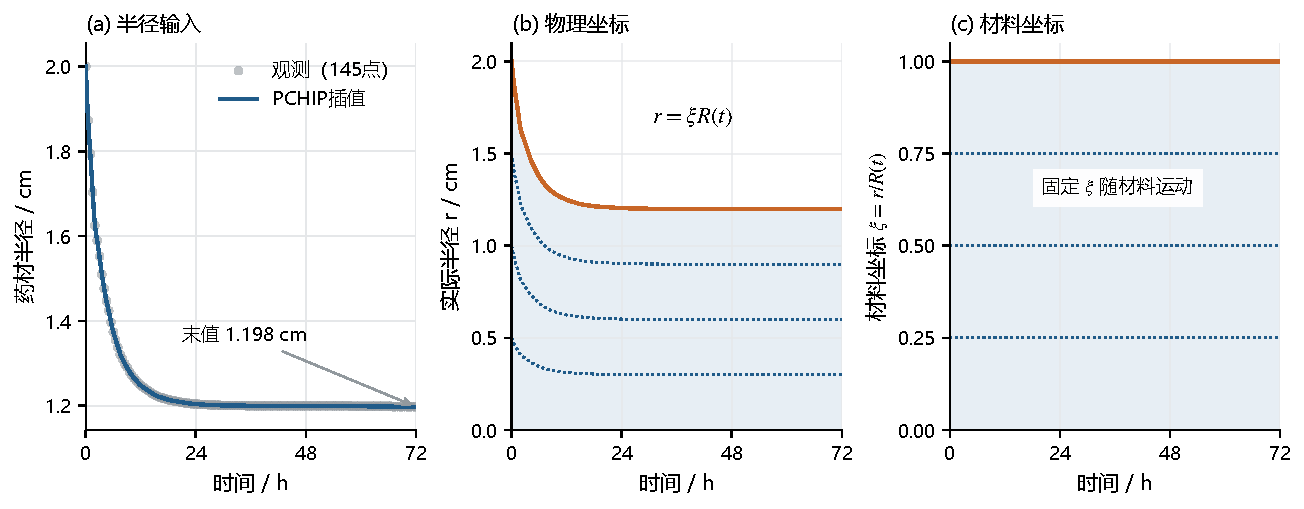
\includegraphics[width=0.98\linewidth]{q4/figures/fig6_q4_radius_mapping.pdf}
\caption{药材收缩半径输入与材料坐标映射}\label{fig:q4-radius}
\end{figure}

\subsection{附录4物性与参考域方程}

第四问从题设均匀初态$t=0$独立计算，全部阶段使用附录4物性。温度$T$在物性公式中采用K；环境温度数据先由摄氏度转换为K。$\rho,c_p,k,D$的单位依次为$\mathrm{kg/m^3}$、$\mathrm{J/(kg\cdot K)}$、$\mathrm{W/(m\cdot K)}$与$\mathrm{m^2/s}$，$C$为干基含水率，单位kg/kg。

\[
\begin{aligned}\rho(C)&=760+90C,\\ c_p(C)&=1850+2150\frac{C}{C+1},\\ k(C)&=0.12+0.20\frac{C}{C+1},\\ D(C,T)&=4.2\times10^{-4}\exp\!\left(-\frac{0.30}{C}\right)\exp\!\left(-\frac{3850}{T}\right).\end{aligned}
\]

材料坐标消去由同比运动产生的显式对流项，径向扩散算子出现$s^{-2}$缩放。本文沿用有效传热传质模型，在$0<x<R_0$上求解

\[
\begin{aligned}\rho(C)c_p(C)\left.\frac{\partial T}{\partial t}\right|_x&=\frac1x\frac{\partial}{\partial x}\left[x\frac{k(C)}{s(t)^2}\frac{\partial T}{\partial x}\right],\\ \left.\frac{\partial C}{\partial t}\right|_x&=\frac1x\frac{\partial}{\partial x}\left[x\frac{D(C,T)}{s(t)^2}\frac{\partial C}{\partial x}\right].\end{aligned}
\]

中心采用对称条件，表面采用与物理域等价的Robin交换条件。将方程通量系数写成$k/s^2$、$D/s^2$时，参考域的对流换热、传质系数必须同时写成$h/s$、$h_m/s$：

\[
\begin{aligned}T_x(0,t)&=C_x(0,t)=0,\\ -\frac{k}{s^2}T_x(R_0,t)&=\frac{h}{s}\bigl(T_s-T_\infty\bigr),\\ -\frac{D}{s^2}C_x(R_0,t)&=\frac{h_m}{s}\bigl(C_s-C_\infty^{\mathrm{eff}}\bigr),\\ T(x,0)&=301.15\ \mathrm{K},\qquad C(x,0)=2.55\ \mathrm{kg/kg}.\end{aligned}
\]

上述$s$因子来自坐标变换，实际物性仍由附录4给定。表面对流系数按既定假设沿用附录2，即$h=25\ \mathrm{W/(m^2\cdot K)}$、$h_m=8\times10^{-7}\ \mathrm{m/s}$。控制体的体积与距离始终采用初始参考几何，缩放仅施加于内部输运和表面交换系数；有效热存储系数仍为$\rho(C)c_p(C)$。

环境输入在0—4 h内采用附件1的分段线性插值，之后采用既定的50.0℃与0.0500 kg/kg恒值延拓。环境水分指标仍按药材侧等效驱动解释。模型不显式计入潜热；经验密度用于热容量。初始干物质分布均匀、各材料壳干物质质量保持不变，因此初始参考体积权重同时给出固定干质量权重，水量收支始终使用这一归一化口径。

\subsection{有限体积离散与水量核对}

参考域使用向表面加密的原生网格，控制体通量在相邻单元间共享；时间推进采用后向Euler全隐式格式与Picard耦合迭代，并同时检查迭代变化与离散残差。每一步在新的绝对时刻评价环境、半径和物性，并对齐输入节点、输出时刻及事件候选时刻。省略所有控制体共有的圆周与长度因子$2\pi\ell$后，径向体积因子及归一化含水率写为

\[
V_j=\frac{x_{j+1/2}^2-x_{j-1/2}^2}{2},\qquad V_0=\sum_jV_j=\frac{R_0^2}{2},\qquad \overline C^n=\frac{\sum_jV_j C_j^n}{V_0}.
\]

记$x_j$为参考控制体中心，$s_{n+1}=s(t_{n+1})$。在新的时刻定义$\widehat D_j=D(C_j^{n+1},T_j^{n+1})/s_{n+1}^2$、$\widehat h_m=h_m/s_{n+1}$，全隐式含水率离散式为

\[
V_j\frac{C_j^{n+1}-C_j^n}{\Delta t_n}=G_{j-1/2}\bigl(C_{j-1}^{n+1}-C_j^{n+1}\bigr)+G_{j+1/2}\bigl(C_{j+1}^{n+1}-C_j^{n+1}\bigr),
\]

\[
G_{j+1/2}=\frac{x_{j+1/2}}{\displaystyle\frac{x_{j+1/2}-x_j}{\widehat D_j}+\frac{x_{j+1}-x_{j+1/2}}{\widehat D_{j+1}}},\quad 1\le j<N;\qquad G_s=\frac{R_0}{\displaystyle\frac{R_0-x_N}{\widehat D_N}+\frac1{\widehat h_m}}.
\]

中心边界取$G_{1/2}=0$；末单元右侧取$G_{N+1/2}=G_s$，并将外侧值替换为$C_\infty^{\mathrm{eff}}(t_{n+1})$。热量方程具有相同通量结构，将$C$替换为$T$，左侧$V_j$替换为$a_jV_j$，其中$a_j=\rho(C_j^{n+1})c_p(C_j^{n+1})$；内部与表面系数分别用$\widehat k_j=k(C_j^{n+1})/s_{n+1}^2$和$\widehat h=h/s_{n+1}$构造，外侧值为$T_\infty(t_{n+1})$。每轮Picard迭代按当前温度、含水率更新物性与上述界面系数，直到状态变化和离散残差同时满足容差。

干基含水率跟随材料位置，不因体积收缩额外乘以$s^{-2}$。采用正向为流出材料的边界水分通量，参考归一化累计失水与收支残差定义为

\[
L(t)=\frac1{V_0}\int_0^t\frac{R_0h_m}{s(\tau)}\bigl[C_s(\tau)-C_\infty^{\mathrm{eff}}(\tau)\bigr]\,\mathrm d\tau,\qquad B(t)=\overline C(t)+L(t)-2.55.
\]

数值累计失水使用实际接受时间步的离散表面通量，与有限体积状态同步累加。本次末态平均含水率为0.1184 kg/kg，累计失水为2.4316 kg/kg；全程最大水量收支残差为9.992007e-13 kg/kg。该残差用于核对所采用离散模型的收支一致性。

\subsection{全域达标判据与实际位置取样}

\[
M_4(t)=\max_{0\le r\le R(t)}C_4(r,t),\qquad g_4(t)=M_4(t)-0.15,\qquad g_4(t_-)\ge0,\quad g_4(t_+)<0.
\]

每个候选时刻检查全部原生单元，并加入中心对称重构值与真实移动表面的Robin重构值，同时记录实际最大值位置。定位采用同一未达标完整锚点的重新积分；严格条件以未舍入的$M_4<0.15$判断，不以固定21个表格点或101个绘图点的最大值替代。

本次严格达标时刻为$t_+=183913.49853515625$ s，即51.0871 h；终点半径为1.2000 cm。实际最大含水率为0.14999999649100706 kg/kg，位置为$r=0.0000$ cm。未达标—达标括区为[183913.4912109375, 183913.49853515625] s，宽度0.00732421875 s。括区宽度表示事件定位分辨率；离散加密差值与其分别核对，不据此宣称未知精确解的总误差上界。

表6按每6 h及精确终点列出固定实际位置$r=0,0.5,1,1.5,2$ cm的含水率，并独立列出表面值。result4.xlsx从60 s开始，以60 s为间隔输出$r=0,0.1,\ldots,2$ cm及真实表面。依据未舍入的半径判断实际位置：对于$r_j>R(t_n)$的位置，Excel、正文表格保留空白，JSON使用null；这些位置属于材料域外。表面列始终取$r=R(t_n)$，不由最外侧固定位置列代替。精确的非整分终点单独保存在终点文件与表6末行。所有取数来自同一份未舍入数值解，表格中的含水率统一作四位小数展示。

\begin{table}[htbp]\centering
\caption{药材干燥过程的干基含水率（kg/kg）}\label{tab:q4-c}
\begin{tabular}{c|rrrrrrr}\hline
时间/h & 0 cm & 0.5 cm & 1 cm & 1.5 cm & 2 cm & 药材表面 & $R(t)$/cm \\\hline
6 & 1.7188 & 1.5370 & 1.0221 &  &  & 0.4205 & 1.3740 \\
12 & 0.7374 & 0.6544 & 0.4082 &  &  & 0.1669 & 1.2480 \\
18 & 0.4086 & 0.3686 & 0.2397 &  &  & 0.0892 & 1.2140 \\
24 & 0.2851 & 0.2610 & 0.1790 &  &  & 0.0673 & 1.2040 \\
30 & 0.2263 & 0.2094 & 0.1493 &  &  & 0.0595 & 1.2010 \\
36 & 0.1928 & 0.1796 & 0.1316 &  &  & 0.0560 & 1.2000 \\
42 & 0.1712 & 0.1604 & 0.1200 &  &  & 0.0541 & 1.2000 \\
48 & 0.1561 & 0.1468 & 0.1116 &  &  & 0.0530 & 1.2000 \\
51.0871（终点） & 0.1500 & 0.1413 & 0.1081 &  &  & 0.0526 & 1.2000 \\
\hline\end{tabular}
\end{table}

\subsection{同物性固定半径对照}

\[
\Delta t_{\mathrm{shrink}\mid\mathrm{A4}}=t_+(\mathrm{A4},R(t))-t_+(\mathrm{A4},R_0).
\]

附录4固定半径对照同样从$t=0$独立求解，采用相同初值与环境边界口径，其严格达标时刻为129.844 h。两组终点的有符号差值为-78.757 h，相对固定对照为-60.655\%。在本组附录4模型条件下，收缩方案的模型终点提前。这一比较限定于同一物性下的几何与同比运动设定；问题3到问题4还同时改变了物性，不能将二者全部时长差异归因于收缩。

用于此处对照的实际数值配置为：收缩组$N=1280$、$\Delta t_{\max}=0.03125$ s；固定组$N=1280$、$\Delta t_{\max}=0.25$ s。各自的加密记录与比较范围在数值验证附录中列明。

两组含水率加密差的核验门槛均为$2\times10^{-5}$ kg/kg；主收缩模型的终点差门槛为0.1 s，固定半径对照的终点差门槛单独取1 s。因此固定对照时长以0.001 h展示。门槛针对所列数值配对的实际差值，不代表未知真解的误差上界。

问题3附录3固定半径模型的终点为57.4723 h。图7将三组模型放在同一物理时间轴下比较；问题3前3 h未保存原生全域最大值，因此对应曲线保留空缺。

\begin{figure}[htbp]\centering
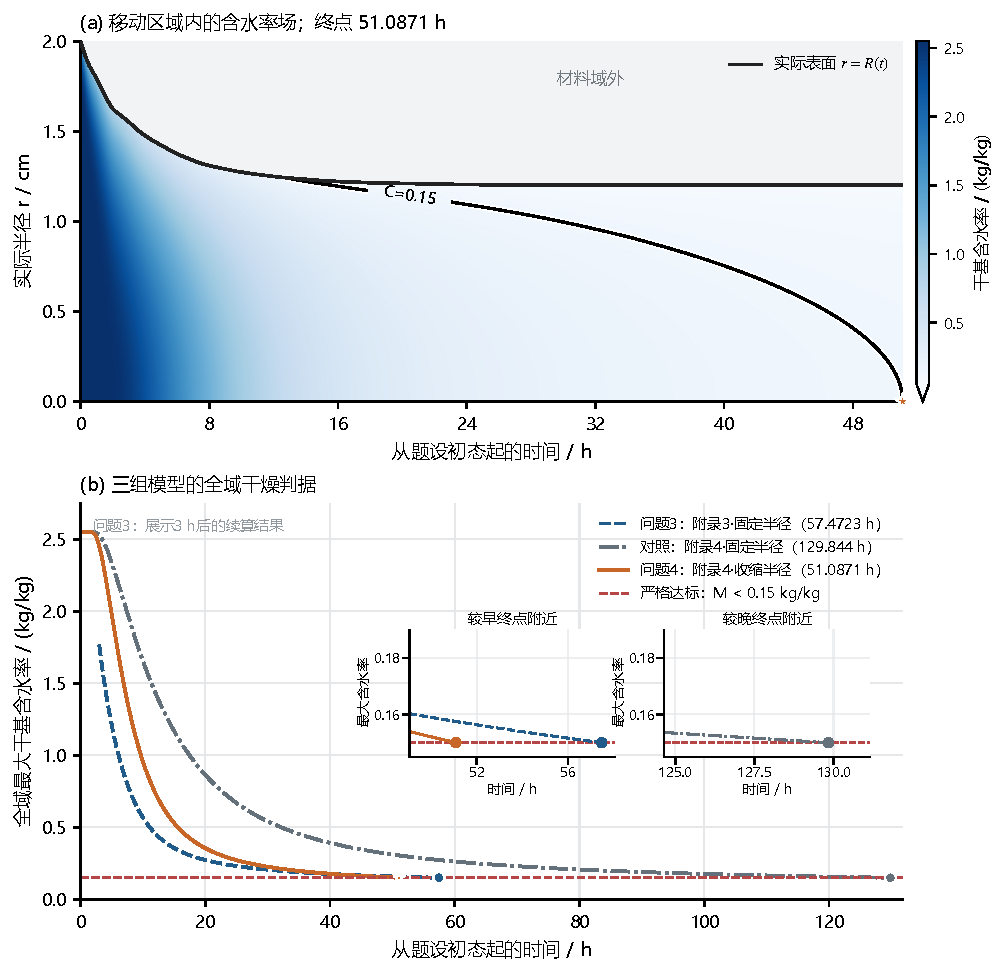
\includegraphics[width=0.98\linewidth]{q4/figures/fig7_q4_shrinking_comparison.pdf}
\caption{移动区域内含水率演化与模型终点对照}\label{fig:q4-field}
\end{figure}

图7的场图由完整参考位置及其实际$r=\xi R(t)$坐标绘制，色块终止于真实表面，材料域外不参与色标、最大值或水量计算。阈值等值线与终点标记使用保存的真实数值；曲线与事件试算不作新根拟合。上述结果是所采用模型的预测与数值复核，附件没有提供内部实测温湿场，因而不将其表述为实验验证。
